\chapter{Cơ sở lý thuyết}
\section{Các cơ sở lý thuyết và công nghệ sử dụng}
\subsection{Reactjs}
\subsubsection{Khái niệm}
\indent ReactJS là một thư viện JavaScript phía người dùng (frontend) được sử dụng để xây dựng giao diện người dùng tương tác \footnote{https://fptcloud.com/reactjs/}.
\subsubsection{Ưu điểm của Reactjs}
\begin{itemize}
    \item \textbf{Tận dụng lại các thành phần có sẵn}

    \indent ReactJS hỗ trợ tích cực trong khởi tạo một website bởi lập trình viên sẽ không cần phải code nhiều như khi tạo trang web mà chỉ sử dụng JavaScript. Đồng thời, nó cung cấp một loạt các thành phần sẵn có mà bạn có thể sử dụng trong nhiều tình huống khác nhau.
    \item \textbf{Tích hợp được cho cả ứng dụng di động Mobile application}

    \indent Hầu hết chúng ta đã biết rằng ReactJS được sử dụng để phát triển các ứng dụng web, tuy nhiên, nó không chỉ giới hạn trong lĩnh vực đó. Nếu chúng ta muốn phát triển các ứng dụng di động, chúng ta có thể sử dụng React Native. Đây là một framework do Facebook phát triển, cho phép chúng ta dễ dàng "chia sẻ" các thành phần và tái sử dụng logic nghiệp vụ trong các ứng dụng của chúng ta.
    \item \textbf{Tối ưu để tăng cường khả năng tìm kiếm SEO}

    \indent Tối ưu hóa công cụ tìm kiếm (SEO) là một yếu tố quan trọng để đảm bảo trang web của chúng ta xuất hiện cao hơn trong kết quả tìm kiếm của Google. ReactJS là một thư viện JavaScript cơ bản. Công cụ tìm kiếm của Google có khả năng thu thập thông tin và lập chỉ mục mã JavaScript, tuy nhiên, nó cũng yêu cầu sự hỗ trợ từ các thư viện khác để làm điều này.
    \item \textbf{Dễ dàng sửa lỗi và gỡ rối Debug}

    \indent Facebook đã phát hành một tiện ích mở rộng Chrome để hỗ trợ việc gỡ lỗi trong quá trình phát triển ứng dụng. Điều này giúp tăng tốc quá trình phát hành sản phẩm cũng như quá trình viết mã của chúng ta.
\end{itemize}
\subsubsection{Nhược điểm của Reactjs}
\begin{itemize}
    \item Reactjs không phải là framework, cho nên chúng ta phải tự xây dựng dự án bằng thủ công.
    \item Tích hợp Reactjs vào các framework MVC truyền thống yêu cầu cần phải cấu hình lại.
    \item Poor Document: Đó là một nhược điểm khá phổ biến đối với các công nghệ cập nhật liên tục. Các công nghệ cập nhật và tăng tốc nhanh đến mức không có thời gian để tạo tài liệu phù hợp.
\end{itemize}
\subsection{Java Spring Boot}

\subsubsection{Khái niệm:} Spring Boot là một framework phát triển ứng dụng Java, dựa trên nền tảng Spring Framework. Nó được thiết kế để giảm bớt công việc cấu hình và cung cấp một cách tiếp cận linh hoạt và nhanh chóng để xây dựng các ứng dụng Java.\footnote{https://lotusacademy.edu.vn/blog/java-spring-boot-la-gi-java-spring-mvc-la-gi-spring-framework-la-gi-256}

\subsubsection{Ưu điểm:}
\begin{itemize}
    \item \textbf{Tự động cấu hình:} Spring Boot tự động cấu hình dựa trên các quy tắc mặc định và cung cấp một số cấu hình tùy chỉnh đơn giản.
    \item \textbf{Tiết kiệm thời gian:} Với Spring Boot, bạn không cần lo lắng về việc cấu hình chi tiết và tập trung vào việc phát triển chức năng của ứng dụng.
    \item \textbf{Tích hợp dễ dàng:} Spring Boot tích hợp tốt với các công nghệ và thư viện phổ biến khác, cho phép bạn dễ dàng tích hợp các thành phần khác như cơ sở dữ liệu, bảo mật, gửi email, vv.
    \item \textbf{Gói hóa ứng dụng:} Spring Boot cho phép bạn gói hóa ứng dụng thành file JAR hoặc WAR, giúp dễ dàng triển khai và chạy trên các môi trường khác nhau.
\end{itemize}

\subsubsection{Nhược điểm:}
\begin{itemize}
    \item \textbf{Phụ thuộc:} Spring Boot có thể tạo ra các ứng dụng có phụ thuộc tăng cao vào framework, điều này có thể làm cho ứng dụng phải dựa vào các phiên bản và cấu hình cụ thể của Spring Boot.
    \item \textbf{Tính linh hoạt:} Mặc dù Spring Boot giảm bớt công việc cấu hình, nhưng đôi khi nó có thể hạn chế tính linh hoạt so với việc cấu hình thủ công bằng XML hoặc Java.
    \item \textbf{Độ phức tạp:} Một số tính năng và cấu hình cao cấp của Spring Boot có thể trở nên phức tạp và khó hiểu đối với những người mới sử dụng.
\end{itemize}
\indent Tuy nhiên, ưu điểm của Spring Boot thường vượt trội hơn so với nhược điểm, vì nó giúp đơn giản hóa việc phát triển và triển khai ứng dụng Java.

\subsection{Nodejs}
\subsubsection{Khái niệm}
\indent Node.js là một môi trường chạy mã JavaScript phía máy chủ, dựa trên JavaScript Engine V8 của Google. Nó cho phép viết mã JavaScript để xây dựng ứng dụng máy chủ một cách hiệu quả. \footnote{https://nodejs.org/en/about}
\subsubsection{Ưu điểm của Node.js:}
\begin{itemize}
    \item Hiệu suất cao: Với JavaScript Engine V8 nhanh chóng, Node.js cho phép xử lý các yêu cầu đồng thời một cách hiệu quả và đạt được hiệu suất cao.
    \item Đơn luồng và không đồng bộ: Node.js sử dụng mô hình xử lý không đồng bộ (non-blocking) I/O, giúp xử lý nhiều yêu cầu cùng một lúc mà không tốn thêm tài nguyên.
    \item Quản lý gói dễ dàng: Node.js có npm (Node Package Manager), cung cấp một kho lưu trữ gói phong phú và dễ quản lý.
    \item Phát triển đồng nhất: Với Node.js, phát triển ứng dụng web và ứng dụng di động có thể được thực hiện bằng cùng một ngôn ngữ và công cụ, tạo sự đồng nhất.
\end{itemize}
\subsubsection{Nhược điểm của Node.js:}
\begin{itemize}
    \item Chưa phù hợp cho các tác vụ nặng: Do Node.js sử dụng mô hình đơn luồng, nó không phù hợp cho các tác vụ tính toán nặng hoặc xử lý dữ liệu lớn.
    \item Đòi hỏi khéo léo trong việc quản lý bộ nhớ: Node.js không tự động quản lý bộ nhớ, điều này yêu cầu phải làm việc thủ công để tránh rò rỉ bộ nhớ.
\end{itemize}
\subsection{Docker}
\subsubsection{Khái niệm:}
\indent Docker là một nền tảng mã nguồn mở giúp đóng gói các ứng dụng và các phụ thuộc của chúng vào những đơn vị gọi là containers. Containers cho phép triển khai một ứng dụng một cách đáng tin cậy và di động với sự độc lập về môi trường.\footnote{https://docs.docker.com/}
\subsubsection{Ưu điểm:}
\begin{itemize}
    \item Đóng gói và triển khai dễ dàng: Docker giúp đóng gói các ứng dụng và phụ thuộc vào một container có thể di chuyển được và triển khai một cách dễ dàng trên nhiều môi trường khác nhau.
    \item Tính nhất quán giữa môi trường phát triển và triển khai: Docker đảm bảo môi trường chạy ứng dụng trên máy chủ phát triển giống với môi trường chạy trên môi trường triển khai.
    \item Hiệu suất cao: Containers Docker nhẹ và nhanh chóng, giúp tối ưu hóa tài nguyên và cung cấp hiệu suất cao cho các ứng dụng.
\end{itemize}
\subsubsection{Nhược điểm:}
\begin{itemize}
    \item Tăng phức tạp: Đôi khi quản lý các container Docker và xử lý các phụ thuộc có thể trở nên phức tạp, đặc biệt là trong các môi trường lớn và phức tạp.
    \item Hiệu suất ảnh hưởng: Mặc dù Docker giúp tối ưu hóa hiệu suất, nhưng việc sử dụng container cũng có thể ảnh hưởng đến hiệu suất so với việc chạy ứng dụng trực tiếp trên máy chủ vật lý.
\end{itemize}

\subsection{Terraform}
\subsubsection{Khái niệm:}
\indent Terraform là một công cụ mã hóa cấu hình (Infrastructure as Code) được sử dụng để tự động hóa việc triển khai và quản lý cơ sở hạ tầng đám mây và hạ tầng điện toán.\footnote{https://www.alibabacloud.com/blog/terraform}
\subsubsection{Ưu điểm:}
\begin{itemize}
    \item Tự động hóa hạ tầng: 
    Terraform cho phép viết mã để mô tả và triển khai cơ sở hạ tầng một cách dễ dàng và nhất quán.
    \item Đa nền tảng: 
    Terraform hỗ trợ nhiều nhà cung cấp đám mây và nền tảng hạ tầng khác nhau như AWS, Azure, GCP, v.v., giúp quản lý và triển khai đồng nhất trên nhiều môi trường.
    \item Kiểm soát phiên bản: 
    Terraform quản lý các tài nguyên hạ tầng như mã nguồn, cho phép theo dõi và quản lý phiên bản tài nguyên trong quá trình phát triển và triển khai.
\end{itemize}
\subsubsection{Nhược điểm:}
\begin{itemize}
    \item Học và quản lý đòi hỏi thời gian: Terraform có độ dốc học đôi khi khá lớn, và việc quản lý mã cấu hình có thể đòi hỏi thời gian và kỹ năng.
    \item Giới hạn của các nhà cung cấp đám mây: Các nhà cung cấp đám mây có thể không hỗ trợ tất cả các tính năng của Terraform hoặc có giới hạn trong việc quản lý hạ tầng.
\end{itemize}
\subsection{Kubernetes}
\subsubsection{Khái niệm:}
\indent Kubernetes (thường được gọi là k8s) là một nền tảng mã nguồn mở để quản lý việc triển khai, tự động hóa và mở rộng ứng dụng container.\footnote{https://kubernetes.io/vi/docs/concepts/overview/what-is-kubernetes/}

\indent Các ứng dụng có sử dụng Kubernetes: Google, Netflix, Airbnb, Spotify, Grab, Zalando, Adidas...và nhiều hơn nữa. Kubernetes đã trở thành một công nghệ phổ biến và mạnh mẽ trong việc quản lý và triển khai ứng dụng quy mô lớn.
\subsubsection{Kiến trúc}
 \begin{figure}[H]
    \begin{center}
    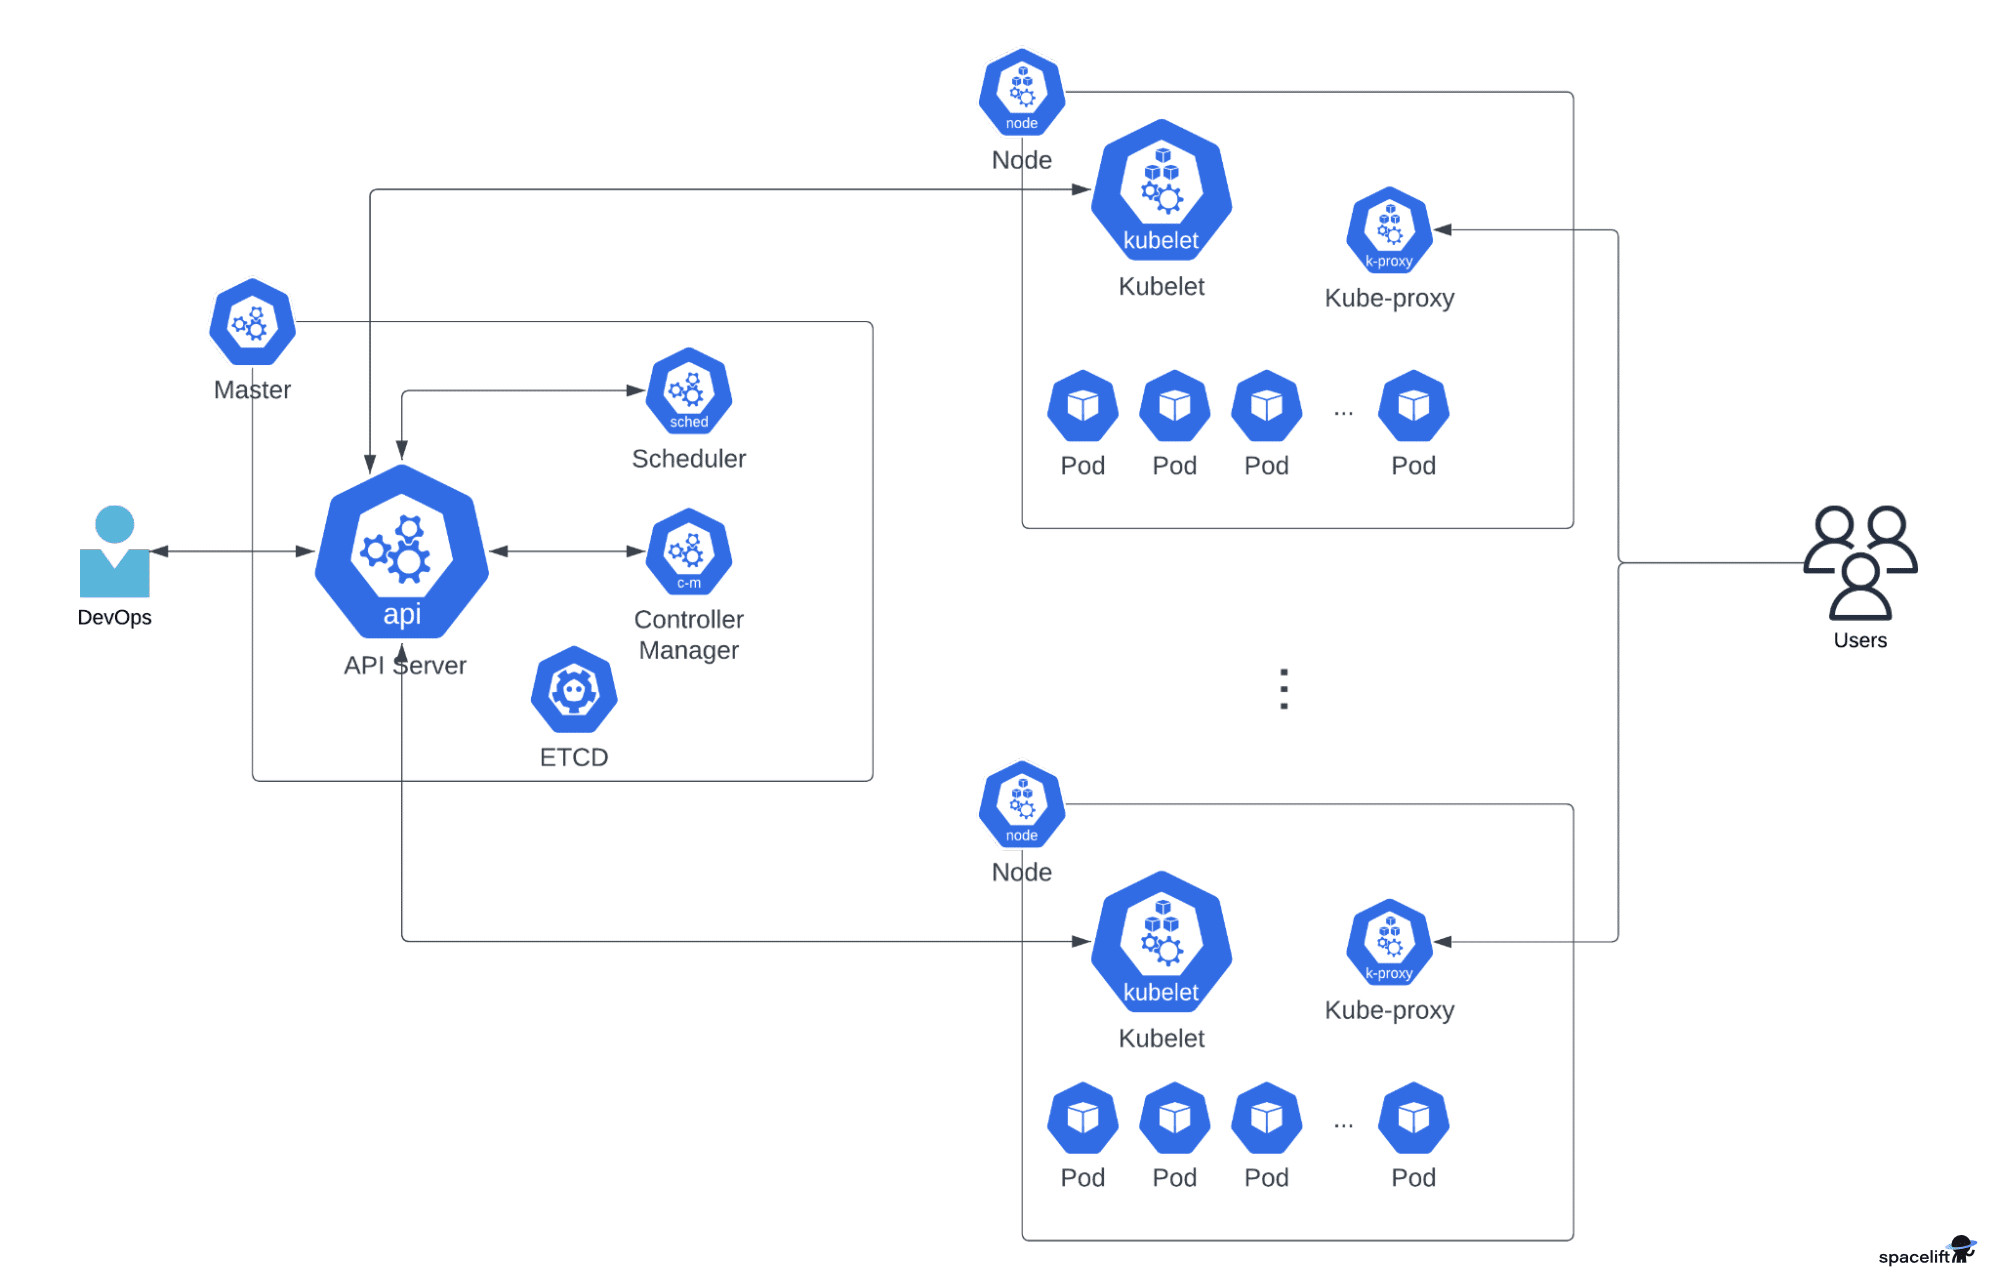
\includegraphics[scale = 0.24]{images/phat/kubernetes_architecture.jpg}
    \vspace*{7mm}
    \caption{Kubernetes Architecture }
    \end{center}
    \label{}
\end{figure}
\indent Kiến trúc của Kubernetes bao gồm:
\begin{itemize}
    \item Master Node: Quản lý, điều phối và giám sát toàn bộ hệ thống Kubernetes.
    \item Worker Node: Chứa các container và chịu trách nhiệm thực hiện các tác vụ đồng bộ từ Master Node.
    \item Pod: Nhóm các container chạy cùng nhau trên cùng một Worker Node, chia sẻ tài nguyên và mạng.
    \item Service: Một tập hợp các Pod có thể truy cập thành một đầu nối duy nhất từ bên ngoài.
    \item Volume: Cung cấp quản lý lưu trữ cho các container trong Pod.
\end{itemize}
\subsubsection{Cách thiết lập Kubernetes cho ứng dụng}
\begin{itemize}
    \item Định nghĩa và triển khai mô tả ứng dụng: Sử dụng các tệp cấu hình (ví dụ: YAML) để định nghĩa ứng dụng, bao gồm Pod, Service và các tài nguyên khác.
    \item Triển khai và quản lý: Gửi yêu cầu triển khai tới Master Node, sau đó Kubernetes sẽ triển khai các Pod và Service, quản lý vòng đời và giám sát.
    \item Tự động mở rộng và cân bằng tải: Kubernetes tự động mở rộng hoặc thu hẹp quy mô của các Pod để đáp ứng tải công việc và cân bằng tải giữa các Worker Node.
\end{itemize}
\subsubsection{Ưu điểm:}
\begin{itemize}
    \item Tự động hóa và quản lý quy mô: Kubernetes cho phép tự động mở rộng và thu hẹp quy mô các thành phần ứng dụng, như các microservice và cụm máy chủ. Điều này giúp tối ưu hóa hiệu suất và đáp ứng đối với lưu lượng truy cập thay đổi.

    \item Đảm bảo sẵn lòng và tin cậy: Kubernetes có khả năng phục hồi lỗi tự động và chuyển đổi dịch vụ giữa các phiên bản trên các nút khác nhau. Điều này giúp đảm bảo rằng ứng dụng luôn sẵn sàng và hoạt động một cách tin cậy.

    \item Quản lý tài nguyên hiệu quả: Kubernetes cung cấp các công cụ quản lý tài nguyên để phân bổ và giám sát tài nguyên phù hợp, bao gồm bộ nhớ, CPU, lưu trữ và mạng. Điều này giúp tối ưu hóa sử dụng tài nguyên và tăng hiệu suất hệ thống.

\end{itemize}
\subsubsection{Nhược điểm:}
\begin{itemize}
    \item Đòi hỏi kiến thức phức tạp: Kubernetes có độ dốc học và quản lý phức tạp, đòi hỏi kiến thức về hạ tầng và kỹ năng quản lý container.
    \item Tài nguyên tốn kém: Kubernetes yêu cầu sự sẵn có của một cụm máy chủ và tài nguyên đáng kể để triển khai và vận hành.
\end{itemize}
\subsection{Redis Cache}
\subsubsection{Khái niệm:}
\indent Redis Cache là một cơ sở dữ liệu key-value (khóa-giá trị) phân tán, được sử dụng để lưu trữ dữ liệu tạm thời trong bộ nhớ. \footnote{https://kdata.vn/cam-nang/redis-la-gi-hieu-ro-ve-he-thong-co-so-du-lieu-trong-bo-nho}
\subsubsection{Ưu điểm:}
\begin{itemize}
    \item Tốc độ và hiệu suất cao: Redis Cache lưu trữ dữ liệu trong bộ nhớ và cho phép truy cập cực kỳ nhanh chóng, đáp ứng yêu cầu với hiệu suất cao.
    \item Đa dạng tính năng: Redis cung cấp nhiều tính năng như caching, xử lý hàng đợi, pub/sub messaging và phân tích dữ liệu, giúp tối ưu hóa các tác vụ dựa trên dữ liệu.
\end{itemize}
\subsubsection{Nhược điểm:}
\begin{itemize}
    \item Giới hạn bộ nhớ: Redis Cache yêu cầu bộ nhớ đủ lớn để lưu trữ dữ liệu. Nếu dữ liệu vượt quá dung lượng bộ nhớ, có thể gặp sự cố và ảnh hưởng đến hiệu suất.
    \item Khả năng mất dữ liệu: Redis Cache mặc định không cung cấp cơ chế đồng bộ hoá dữ liệu, điều này đồng nghĩa rằng có thể mất dữ liệu khi xảy ra sự cố.
\end{itemize}
\subsection{PostgreSQL}
\subsubsection{Khái niệm:}
\indent PostgreSQL (viết tắt là Postgres) là một hệ quản trị cơ sở dữ liệu quan hệ mã nguồn mở, được đánh giá là ổn định, mạnh mẽ và có tính mở rộng.
\subsubsection{Ưu điểm:}
\begin{itemize}
    \item Độ tin cậy cao: PostgreSQL được thiết kế để đảm bảo tính toàn vẹn và độ tin cậy của dữ liệu, bao gồm các tính năng như ACID và khả năng khôi phục dữ liệu.
    \item Tính mở rộng và phân vùng: PostgreSQL hỗ trợ phân vùng dữ liệu và khả năng mở rộng sẵn sàng, cho phép mở rộng cơ sở dữ liệu để xử lý lượng dữ liệu lớn và tải cao.
    \item Đa dạng tính năng: PostgreSQL cung cấp nhiều tính năng tiên tiến bao gồm trình tự, trigger, tìm kiếm văn bản và hình ảnh, và hỗ trợ các loại dữ liệu phong phú.
\end{itemize}
\subsubsection{Nhược điểm:}
\begin{itemize}
    \item Có thể cảm thấy phức tạp đối với các dự án nhỏ.
\end{itemize}
\subsection{EKS}
\subsubsection{Khái niệm:}
\indent EKS (Elastic Kubernetes Service) là một dịch vụ quản lý Kubernetes do Amazon Web Services (AWS) cung cấp.
\subsubsection{Ưu điểm:}
\begin{itemize}
    \item Dễ dàng triển khai, quản lý và mở rộng các ứng dụng chạy trên Kubernetes.
    \item Tích hợp tốt với dịch vụ AWS khác.
    \item Hỗ trợ cho môi trường đám mây tiêu chuẩn và quy mô lớn.
\end{itemize}
\subsubsection{Nhược điểm:}
\begin{itemize}
    \item Phí sử dụng có thể cao, đặc biệt trong trường hợp triển khai lớn.
    \item Đòi hỏi kiến thức về quản lý và triển khai hệ thống phức tạp hơn so với các giải pháp khác.
\end{itemize}
\subsection{AKS}
\subsubsection{Khái niệm:}
\indent AKS (Azure Kubernetes Service) là một dịch vụ quản lý Kubernetes.

\subsubsection{Ưu điểm:}
\begin{itemize}
    \item Dễ dàng triển khai, quản lý và mở rộng các ứng dụng chạy trên Kubernetes.
    \item Tích hợp tốt với dịch vụ Azure và công cụ phát triển của Microsoft.
    \item Cung cấp tính năng bảo mật và giám sát mạnh mẽ.
\end{itemize}
\subsubsection{Nhược điểm:}
\begin{itemize}
    \item Phí sử dụng có thể cao, đặc biệt trong trường hợp triển khai lớn.
    \item Yêu cầu sử dụng môi trường và công cụ phát triển Azure.
\end{itemize}
\subsection{RabbitMQ}
\subsubsection{Khái niệm:}
\indent RabbitMQ là một hệ thống message broker mã nguồn mở, dựa trên giao thức AMQP (Advanced Message Queuing Protocol).
 \begin{figure}[H]
    \begin{center}
    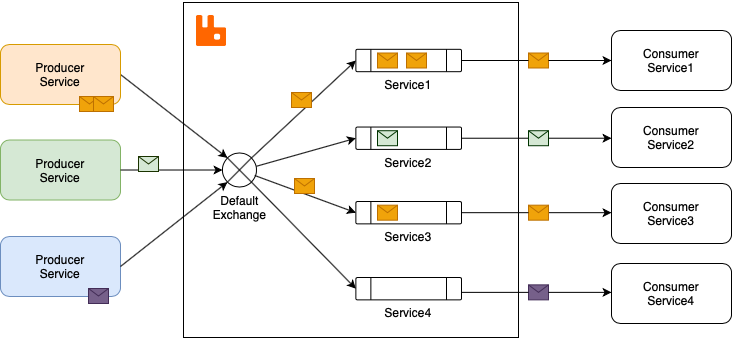
\includegraphics[scale = 0.5]{images/phat/rabbitMQ.png}
    \vspace*{7mm}
    \caption{RabbitMQ Architecture}
    \end{center}
    \label{}
\end{figure}
\subsubsection{Kiến trúc của RabbitMQ}
\begin{itemize}
    \item Producer:

Là thành phần tạo ra và gửi các thông điệp (message).
Message được gửi đến một exchange.
    \item Exchange:

Nhận thông điệp từ nhà sản xuất và định tuyến chúng đến hàng đợi (queue) thích hợp.
Có các loại định tuyến khác nhau như direct, topic, fanout, và headers, cho phép định tuyến dựa trên các tiêu chí khác nhau.
    \item Queue (Hàng đợi):

Là nơi lưu trữ các thông điệp đến từ sàn giao dịch cho đến khi chúng được xử lý bởi một tiêu thụ (consumer).
Các hàng đợi có thể được chia sẻ giữa nhiều tiêu thụ hoặc có thể chỉ được sử dụng bởi một tiêu thụ cụ thể.
    \item Binding (Ràng buộc):

Liên kết giữa một exchange và một queue, xác định cách thông điệp nên được định tuyến từ exchange đến queue.
Ràng buộc này được thiết lập thông qua các quy tắc định tuyến (routing key).
    \item Consumer:

Là thành phần đọc và xử lý các thông điệp từ hàng đợi.
Có thể có nhiều tiêu thụ cùng một lúc đọc từ cùng một hàng đợi.
    \item Virtual Host:

Là một không gian làm việc ảo trong RabbitMQ, giúp tách biệt và cô lập các ứng dụng và người dùng khác nhau.
Mỗi Virtual Host có thể có các exchange, queue, và quyền riêng biệt.
    \item Broker:

Là nền tảng hoạt động của RabbitMQ.
Nhận thông điệp từ nhà sản xuất, định tuyến chúng đến hàng đợi thông qua sàn giao dịch và chuyển giao chúng đến các tiêu thụ.
    \item Connection:

Là một kết nối mạng giữa ứng dụng và RabbitMQ Broker.
Mỗi ứng dụng có thể có nhiều kết nối.
\end{itemize}

\subsubsection{Ưu điểm:}
\begin{itemize}
    \item Hỗ trợ đa ngôn ngữ và dễ dàng tích hợp với các ứng dụng phổ biến.
    \item Cung cấp tính năng đám mây phân tán, đảm bảo bất đồng bộ và xử lý hàng đợi.
    \item Tích hợp tốt với các công nghệ và framework khác như Spring, .NET, Node.js, etc.
\end{itemize}
\subsubsection{Nhược điểm:}
\begin{itemize}
    \item Cấu hình phức tạp và yêu cầu kiến thức về hệ thống phân tán.
    \item Hiệu suất có thể bị ảnh hưởng đối với tải công việc rất cao.
\end{itemize}